\ch{Concept and Methodology}{concept} 

In order to address the identified gap, this thesis proposes the development methodology for an autonomous environment capable of executing complex, multi-step workflows from free-form NL instructions. Although various domains could be used to demonstrate this methodology, the implementation and validation were conducted within an electrochemistry-focused SDL. This use case was selected for its ability to assist scientists, student assistants, and laboratory engineers without requiring prior experience in industrial robot programming or control, as illustrated in Figure~\ref{fig:labtechnicanoperator} \cite{teachpendant, app13042582, quigley2009ros, angerer2010robotics}. Its structured yet diverse experimental routines provide an ideal benchmark for validating autonomous control frameworks that integrate precise robotic motion with analytical measurement tasks, enabling the automation of experiments that would otherwise be time-consuming if performed manually.

The proposed system architecture integrates a multi-purpose robotic manipulator for executing pick-and-place operations and a precision measurement instrument capable of acquiring multiple forms of electrochemical data. At its core, an LLM functions as the high-level planner, transforming unstructured user objectives expressed in NL into structured, executable tool calls \cite{doi:10.1177/1729881419851402, LAURIA2002171, wang2025function}. This design enables seamless translation of human intent into coordinated robotic and analytical actions within the autonomous laboratory environment.

This chapter establishes the conceptual and methodological foundation of the proposed autonomous laboratory. \textbf{Section~\ref{sec:architecture}} introduces the overall system concept and architecture, outlining the hierarchical control flow between the user, AI Agent, and the physical laboratory components. \textbf{Section~\ref{sec:methodological}} presents the methodological approach, describing the integration of the \texttt{smolagents} framework with the hardware control stack and detailing the abstraction from low-level motion primitives to high-level autonomous tasks. Together, these sections provide the structural and procedural basis for a verifiable, fully operational SDL governed by an AI Agent.


\sect{System Concept / Architecture}{architecture} 

As illustrated in Figure~\ref{fig:system_architecture}, the overall architecture consists of a hierarchical control flow linking the user, the AI Agent, and the physical SDL components. The user communicates through unstructured NL instructions, which are processed by the AI Agent guided by a predefined system prompt and an LLM. The agent interprets the input, performs reasoning and planning, and issues executable tool calls to the respective hardware modules such as the robotic manipulator and the measurement device. The acquired data are subsequently stored in a structured database, and NL feedback is generated for the user to close the interaction loop.

\begin{figure}[H]
    \centering
    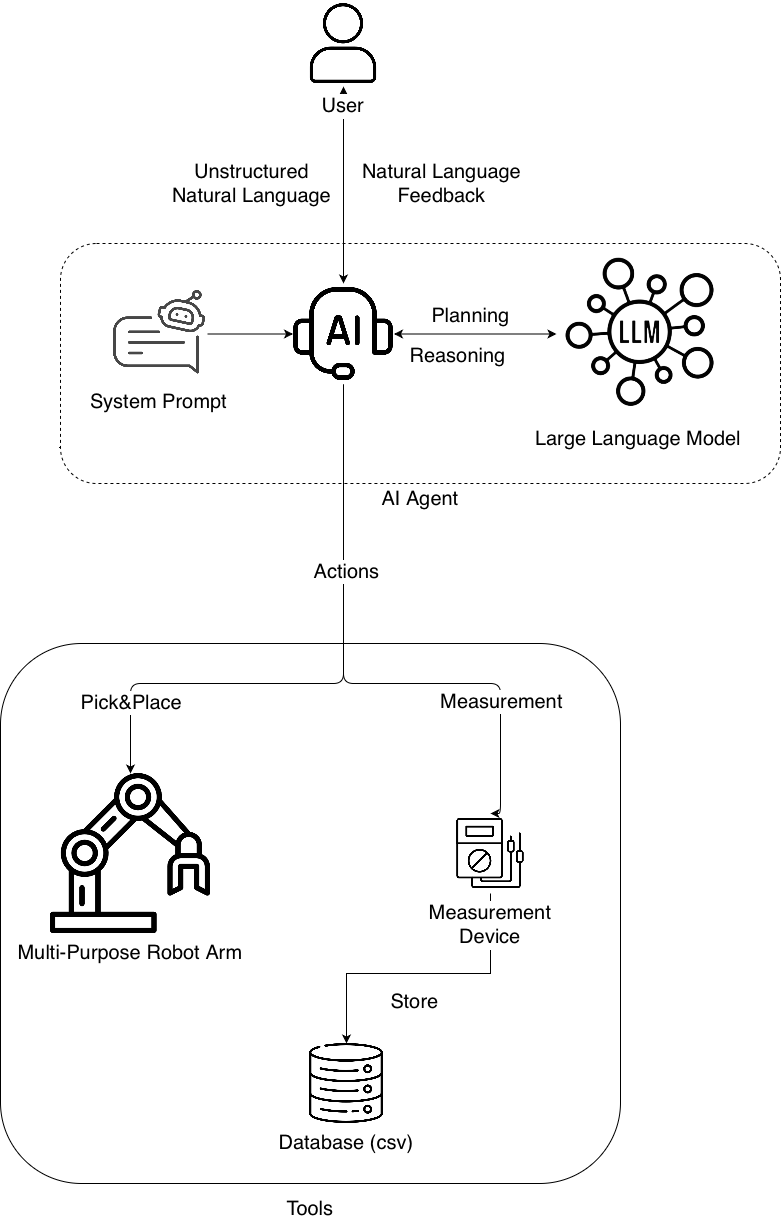
\includegraphics[width=0.7\linewidth]{Images/systemconcept.png}
    \caption{System Concept Architecture of the Proposed SDL}
    \label{fig:system_architecture}
\end{figure}

As illustrated in the system architecture diagram, the core components of the proposed framework are defined as follows:

\begin{itemize}
    \item \textbf{Robotic Arm:} Responsible for physical manipulation, sample transfer, and interaction with laboratory hardware.
    \item \textbf{Measurement Instruments:} Devices used to perform experimental measurements and acquire quantitative data.
    \item \textbf{Database:} A structured data repository for storing, organizing, and retrieving experimental results.
    \item \textbf{AI Agent:} The central control unit that interprets user instructions, plans experimental sequences, and coordinates all system components.
\end{itemize}

Another central aspect of this work is the design and implementation of the AI Agent itself. The core components of the agent are defined by two primary elements: the LLM selected as the reasoning engine and the system prompt that establishes its operational context, boundaries, and objectives. The configuration of these two elements determines the agent’s interpretive capability, response accuracy, and overall behavior within the autonomous laboratory environment.

The user interacts with the AI Agent through a web-based chat interface, submitting NL queries in textual form. This interface serves as the primary communication channel between the human operator and the autonomous system, enabling direct task initiation, progress monitoring, and feedback retrieval without requiring any prior knowledge of robotic control or programming.

Upon receiving a user query, the AI Agent performs a reasoning process to interpret the instruction and determine the appropriate sequence of actions. It then executes the corresponding tools available within its environment. Each tool represents a high-level function composed of multiple low-level routines, such as commanding the robotic arm to a specific position or initiating a measurement procedure. This hierarchical structure ensures modularity, clarity of execution, and reliable control over both mechanical and analytical subsystems of the SDL.

After the execution of the functions within the invoked tools, the resulting data are automatically stored in a comma-separated values (CSV) file, which serves as the system’s structured database. This file-based storage approach enables straightforward data logging, retrieval, and post-processing while maintaining compatibility with common data analysis frameworks. Each entry in the database includes the executed tool, associated parameters, measurement results, and timestamps to ensure complete traceability of all experimental actions. A file-based storage model was favored over database servers to simplify portability, maintain transparency in logged data, and facilitate offline analysis without additional dependencies.

At the conceptual level, users are gonna interact with the AI Agent through written inputs that correspond to specific laboratory tasks. Example queries include:

\begin{itemize}
    \item ``Take this sample from me and place it in the third slot of the sample base.''
    \item ``Measure the open-circuit potential (OCP) value of the third sample, then measure the chronoamperometry (CA) value.''
    \item ``Bring the third sample to the user area.''
\end{itemize}

These examples illustrate the intended mode of interaction, where unstructured user input is interpreted by the agent and translated into structured tool executions within the SDL environment.

Since each tool is implemented as an independent and discrete software module, new tools can be added, modified, or removed without altering the overall system architecture. The only required adjustment in such cases is the update of the system prompt, which informs the AI Agent about the available toolset and their corresponding functionalities.

The proposed approach of automating the SDL through an AI Agent represents a deviation from conventional automation frameworks. In contrast to rigid, task-specific systems, this architecture is inherently scalable and adaptable to new experimental configurations. Its modular structure and language-driven control paradigm allow seamless integration of additional tools or instruments, making the methodology broadly applicable across different types of autonomous environments.


\sect{Methodological Approach}{methodological} 


In this work, an LLM was employed for agentic purposes, serving as the core reasoning component responsible for interpreting user instructions and coordinating experimental actions. The objective was to evaluate the feasibility of enabling autonomous laboratory control through NL understanding and structured function execution.

Two methodological approaches were explored. The first approach involved using a bare LLM directly through structured prompting to perform controlled function calls, effectively forming a handcrafted automation pipeline. While this method provided full transparency and control, it proved less efficient and more complex to maintain, particularly when scaling to multiple tools and task sequences. 

The second approach utilized a dedicated agent framework, \texttt{smolagents} \cite{huggingface_smolagents_good_agents, datacamp_smolagents_guide, towardsai2024comparison}, which natively supports tool registration, reasoning loops, and structured execution. This framework significantly simplified implementation by handling prompt formatting, function invocation, and error recovery within a unified architecture. Owing to its modularity, stability, and ease of integration, the \texttt{smolagents}-based configuration was adopted as the primary methodology for this work. Compared to alternative frameworks such as LangChain or custom-built orchestration pipelines, \texttt{smolagents} was chosen for its lightweight architecture, native function registration, and reliable code writing, which are the features essential for an AI Agent. \cite{openai2023practicalagents, towardsai2024comparison}.

To ensure consistent, reliable interpretation of free-form natural-language instructions, the system prompt needs to be designed following prompt-engineering best practices as outlined by Khatami \& Frantz \cite{khatami2024prompt}. The prompt needs to explicitly assigns the agent a specialist role, outlines the available tool-set, and requires responses strictly in a structured format with no additional explanatory text. Furthermore, the prompt must also prevent data loss, added assumptions, and unclear or nested commands. This helps the LLM agent follow user instructions exactly and call the right tools.

The adopted \texttt{smolagents}-based implementation employs the \texttt{CodeAgent} class in combination with the \texttt{LiteLLMModel} as the reasoning engine \cite{openai_litellm_agents_sdk}. The developed agentic SDL controllers interface directly with the defined tools, which represent the functional abstractions of the physical components such as the measurement instruments and the robotic arm (uFactory xArm 6). Each tool corresponds to a Python function derived from the motion orchestration and respective hardware APIs, enabling precise control over individual laboratory actions. By sequencing multiple low level tasks within higher-level functions, the system can execute complete experimental workflows, such as measuring a specific parameter for the $i$-th sample, through a single user instruction.

In the proposed approach, the robotic arm constitutes a central component of the autonomous system. Initially, all low-level motion commands were implemented through the manufacturer’s Python API, including fundamental operations such as moving to specific coordinates, opening or closing the gripper, and returning to the home position. Although the overall system architecture was designed to enable high-level autonomy, conventional robot programming interfaces, as discussed in Section~\ref{sec:classicalprogramming}, remained essential for implementing and validating the underlying low-level motion control routines. Building upon these primitives, mid-level functions were developed to perform semantically meaningful operations such as picking up a sample from the base, placing it in the measurement area, or retrieving it after a completed measurement. However, these mid-level functions alone remain too granular to be treated as tools within the agentic framework. Therefore, a set of high-level functions was introduced, each representing the maximum atomic task the robot can execute autonomously without requiring additional context or user input. This abstraction allows the AI Agent to complete complex physical actions, such as a full pick-and-place sequence, through a single function call rather than a chain of multiple low-level commands, improving both efficiency and reliability in execution. This abstraction was introduced after observing that direct LLM control over primitive motion commands led to inconsistent spatial reasoning and excessive prompt context requirements, thus necessitating a hierarchical function structure.

For instance, a standard low-level motion command for directing the robotic arm to a specific position is shown below. Such instructions define the exact spatial coordinates and orientation parameters for the robot end-effector, as well as motion characteristics such as speed, path radius, and synchronization behavior. These commands form the foundation of the higher-level motion primitives used in the SDL control architecture.

\begin{lstlisting}[language=Python, caption={Lowest Level Positioning of uFactory xArm 6 for Single Position}]
uFactory_xArm.arm.set_position(x=-742, y=-229, z=162, roll=90, pitch=0, yaw=-90, speed=300, radius=20, wait=True)
\end{lstlisting}

Therefore, it is impractical for the AI Agent to generate and sequence every individual motion command required for a complete task, as this would demand extensive context and precise spatial reasoning beyond its scope. To address this limitation, multiple low-level operations were consolidated into intermediate, task-oriented functions that encapsulate complete pick-and-place actions \cite{cambon2009hybrid, semanticmaps}. These mid-level functions enable the robot to perform coherent physical tasks such as collecting a sample from the user area and placing it into a predefined slot within the sample base. An example implementation of such a function for picking a sample from the user is presented below:

\begin{lstlisting}[language=Python, caption={Middle Level Pick\&Place Task of uFactory xArm 6}]
def pick_sample_from_userarea():
    print("Picking sample from user area...")
    uFactory_xArm.move_to(uFactory_xArm.offsethome)
    uFactory_xArm.arm.set_position(x=263,y=0,z=185,roll=180,pitch=0,yaw=0,
                    speed=300, radius=20, wait=False)   # 20 mm blend
    uFactory_xArm.arm.set_position(x=45,y=-270,z=215,roll=180,pitch=0,yaw=-120,
                    speed=300, radius=20, wait=False)    # stop at final
    uFactory_xArm.arm.set_position(x=-250,y=-85,z=300,roll=180,pitch=0,yaw=-160,
                    speed=300, radius=20, wait=False)    # stop at final
    uFactory_xArm.arm.set_position(x=-742,y=-229,z=162,roll=90,pitch=0,yaw=-90,
                    speed=300, radius=20, wait=True)   
    uFactory_xArm.gripper_open()
    uFactory_xArm.move_to(uFactory_xArm.userarea)
    uFactory_xArm.gripper_close()
    uFactory_xArm.arm.set_position(x=-742,y=-229,z=162,roll=90,pitch=0,yaw=-90,
                    speed=300, radius=20, wait=True)   
    uFactory_xArm.arm.set_position(x=-250,y=-85,z=300,roll=180,pitch=0,yaw=-160,
                    speed=300, radius=20, wait=False)    # stop at final
    uFactory_xArm.arm.set_position(x=45,y=-270,z=215,roll=180,pitch=0,yaw=-120,
                    speed=300, radius=20, wait=False)    # stop at final
    uFactory_xArm.arm.set_position(x=263,y=0,z=185,roll=180,pitch=0,yaw=0,
                    speed=300, radius=20, wait=False)   # 20 mm blend
    uFactory_xArm.move_to(uFactory_xArm.offsethome)
\end{lstlisting}

As demonstrated, defining higher-level motion functions substantially simplifies task execution, as each complete operation can be invoked through a single function call rather than a sequence of individual low-level commands. This abstraction improves readability, maintainability, and reliability within both the control code and the AI Agent’s function-calling logic.

At higher levels of abstraction, generating complex motion sequences directly through an LLM becomes increasingly impractical, since end-user instructions are typically expressed in NL with broad intent rather than detailed procedural steps (e.g., “Can you pick up this sample from me and place it in the third slot?”). To enable the agent to interpret and execute such commands effectively, the final tool layer must encapsulate all underlying operations required to complete the task autonomously. The following function illustrates this concept by integrating all necessary motion primitives for collecting a sample from the user area and placing it into a specified slot on the sample base:

\begin{lstlisting}[language=Python, caption={High-Level Automated Workflows in one Single Function}]
def collect_sample_from_user(i: int) -> Observation:
    obs = start_obs(step="interaction", tool="collect_sample_from_user", args={"i": i})
    try:
        uFactory_xArm.pick_sample_from_userarea()
        uFactory_xArm.place_sample_to_bed(i)
        obs = finish_ok(obs, sample=i, extra_meta={"source": "userarea"})
    except Exception as e:
        obs = finish_err(obs, e)
    finally:
        log_observation(obs)
    return obs
\end{lstlisting}

This high-level function represents the maximum autonomous operation of the robotic subsystem that can be triggered through a single agentic call, ensuring that each user query corresponds to one complete, context-aware laboratory action.

With the robotic subsystem fully implemented, the next component of the SDL concerns the measurement instruments. In this setup, an electrochemical measurement device, the potentiostat, is employed as the primary analytical instrument. The device provides a programmable Python interface that allows direct control and execution of measurement routines through scripting. Using this interface, the system is capable of performing various electrochemical analyses; however, for the scope of this study, three measurement types were selected as representative cases: open-circuit potential (OCP), chronoamperometry (CA), and cyclic voltammetry (CV).

After preparing all tool modules, the \texttt{CodeAgent}, \texttt{LiteLLMModel}, and \texttt{GradioUI} components were imported into the \texttt{labagent} module to establish the complete agentic control structure.

\begin{itemize}
    \item \textbf{\texttt{CodeAgent}:} Serves as the central coordination layer of the agent, managing reasoning loops, tool invocation, and structured execution of tasks. It interprets user input, determines the required tool sequence, and monitors the success or failure of each action \cite{huggingface_smolagents_docs}.

    \item \textbf{\texttt{LiteLLMModel}:} Provides the language model interface responsible for NL understanding, reasoning, and generation. It processes the user’s textual queries, produces the corresponding structured actions, and ensures compatibility with the local \texttt{Ollama}-based LLM backend \cite{openai_litellm_agents_sdk}.

    \textbf{\texttt{GradioUI}:} Implements a lightweight web-based user interface (UI) that enables direct interaction with the agent \cite{gradio_llm_agents}. It allows users to enter NL commands, visualize responses, and observe real-time system behavior during experimental execution.

\end{itemize}

After completing the integration of the agent framework components, the next step was the selection of the language model. The \texttt{Qwen2.5-Instruct} model \cite{qwen_qwen2.5-7B-Instruct, qwen2.5_blog} was chosen for this implementation due to its strong instruction-following capability, efficient local deployment performance, and compatibility with the \texttt{Ollama} backend. Its balance between computational efficiency and reasoning accuracy makes it suitable for continuous operation in a local laboratory environment without dependence on external cloud services. The \texttt{Qwen2.5-Instruct} model was selected over other open-weight alternatives such as \texttt{Mistral} or \texttt{LLaMA-3} due to its superior instruction-following consistency, reduced VRAM footprint, and efficient inference under the \texttt{Ollama} runtime \cite{liduos_open_source_ai_models_2025}.
Local deployment was also prioritized to guarantee low-latency response and data privacy within the laboratory network.


Once the agent’s structural components were finalized, a system prompt was defined to establish the behavioral context and functional boundaries of the AI Agent. The system prompt specifies the agent’s purpose, the available tools, and the correct usage syntax for each tool. This configuration enables the framework to interpret user inputs such as “Measure the OCP of the first sample” and translate them into corresponding structured tool calls, for example, \texttt{measure\_ocp(i=1)}. As a result, each NL query from the user can be executed deterministically through a single, well-defined function invocation within the SDL.

All measurement results are stored in structured files to ensure data traceability and reproducibility. To manage this data layer more effectively, a secondary agent was conceptualized for analyzing recorded results and facilitating information exchange with the user regarding the accumulated dataset. This data-oriented agent was implemented using the same architectural foundation as the main control agent, enabling it to query, summarize, and communicate experimental outcomes in NL. However, since the design and evaluation of a multi-agent framework extend beyond the primary scope of this study, the integration of this secondary agent will be further explored in future work.

The validation aimed to assess the interpretive reliability, task execution accuracy, and operational robustness of the proposed LLM-guided control framework. For that two complementary evaluation stages were designed. First, a simulation-based analysis using 150 structured queries tested the deterministic reasoning and function-calling correctness under controlled conditions. Second, a real-user evaluation with 5 participants, who given a user briefing document for educating them about the Agent and the SDL, examined natural instruction variability, interaction latency, and success rate within the physical SDL setup. The resulting metrics, which is mainly execution success, served to quantify the system’s effectiveness and to verify its ability to autonomously translate natural-language instructions into reproducible robotic actions. Task success was measured by comparing the outputs. A match meant the Agent chose the correct tools and completed the task as intended. A mismatch meant the Agent misunderstood the instruction or produced the wrong result due to system or SDL limitations.


To validate the proposed software architecture and the methodology, a fully operational SDL was required. Therefore, following the completion of the conceptual design phase, the development proceeded with the detailed product design, manufacturing, and assembly of the physical SDL setup. This included the fabrication of mechanical components, integration of electronic and measurement subsystems, and final deployment of the developed software framework onto the assembled system for experimental validation.

